\documentclass[12pt, a4paper]{article}

\usepackage[czech]{babel}
\usepackage[T1]{fontenc}
\usepackage[utf8]{inputenc}
\usepackage{enumitem}
\usepackage{parskip}
\usepackage{tocloft}
\usepackage[hidelinks]{hyperref}
\usepackage{graphicx}
\usepackage{float}
\usepackage[table,xcdraw]{xcolor}
\usepackage{pdflscape}

\newcommand{\Subject}{KIV/UPS}
\newcommand{\TypeOfWork}{Semestrální práce}
\newcommand{\WorkFor}{\Subject\- -- \TypeOfWork}
\newcommand{\NameOfProject}{Síťová aplikace hry Kostky(Farkle)}
\newcommand{\Autor}{Martin Schön}
\newcommand{\Id}{A22B0144P}
\newcommand{\Date}{\today}


\begin{document}

\begin{titlepage}
    \begin{center}
        
        
\includegraphics[width=\textwidth]{Images/fav.pdf}
        
        \vspace{2cm}
        
        \huge
        \textbf{\WorkFor}
        
        \vspace{1cm}
        
        \huge
        \NameOfProject
        
        \vfill
        
        \vspace{0.5cm}
        
        \normalsize
        \raggedright
        Vypracoval: \Autor \\
        Studijní číslo: \Id \\
        Datum: \Date
        \vspace{0.2cm}
        
    \end{center}
\end{titlepage}
\thispagestyle{empty}
\pagebreak

%tečky v~obsahu
\renewcommand{\cftsecleader}{\cftdotfill{\cftdotsep}}
\renewcommand{\cftsubsecleader}{\cftdotfill{\cftdotsep}}
\renewcommand{\cftsubsubsecleader}{\cftdotfill{\cftdotsep}}

%obsah
\setcounter{page}{2}
\tableofcontents
\newpage

\section{Zadání}
Hlavní cíle práce:
\begin{itemize}
    \item Síťová hra pro více hráčů, architektura server-klient (1:N), PC
    \item Server: C/C++
    \item Klient: Java, C\# (i např. Unity), Kotlin nebo jiný vysokoúrovňový jazyk (musí schválit cvičící)
\end{itemize}
Varianty zadání:
\begin{itemize}
    \item tahová hra (prší, mariáš, šachy, piškvorky, ...)
    \item real-time hra (různé skákačky a~střílečky, tanky, "Bulánci", ...)
    \item pseudo-real-time (Pong, Arkanoid, ...)
\end{itemize}

Požadavky na protokol:
\begin{itemize}
    \item textový protokol nad transportním protokolem TCP nebo UDP
    \begin{itemize}
        \item při shodě zadání v~rámci cvičení (max. 2) bude každý student používat jiný
    \end{itemize}
    \item bez šifrování
    \item využijte znalostí ze cvičení při návrhu (např. transparentnost při přenosu dat, apod.)
    \item když se nic neděje (žádný hráč nic nedělá), nic se neposílá
    \begin{itemize}
        \item výjimkou může být občasná ping zpráva
    \end{itemize}
    \item na každý požadavek přijde nějaká reakce (byť by šlo pouze o~jednoznakové potvrzení, že se operace podařila)
\end{itemize}

Celé zadání je dostupné zde: \\ \url{https://home.zcu.cz/~ublm/files/PozadavkyUPS.pdf}.

\section{Zvolená varianta}
Server je implementován v~jazyce C++ a~klient je implementován v~jazyce Java. 
Jako hra byla zvolena hra Kostky (Farkle) inspirovaná minihrou ze hry \textbf{Kingdome Come: Deliverance}. 
Hra je tahová pro dva hráče. 

Byl využit textový protokol nad transportním protokolem TCP.

\newpage

\section{Popis hry}
Hra Kostky (Farkle) je hra pro dva hráče, kteří se střídají v~tazích.
Každý tah hráč hodí šest kostek a~podle výsledku hodů získává body.
Hráč po každém hodu může vybrat, které kostky si nechá a~které hodí znovu.
Hráč se může rozhodnout bude-li házet znovu anebo si ponechá body z~tohoto tahu.
Pokud hráč vybral všechny kostky, může hodit znovu všechny šest kostek.
Pokud hráč hodí a~nezíská žádné body, ztrácí všechny body z~tohoto tahu a~je na tahu druhý hráč.
Hra končí, když jeden z~hráčů dosáhne 4000~bodů.

Kombinace kostek, které hráč může získat a~libovolně kombinovat.
Kombinace s~vyšší hodnotou jsou mají vyšší priority.

\begin{table}[H]
    \centering
    \resizebox{\textwidth}{!}{
    \begin{tabular}{|
    >{\columncolor[HTML]{C0C0C0}}c |c|c|c|c|c|c|}
    \hline
    \textbf{\(\frac{\times}{value}\)} & \cellcolor[HTML]{C0C0C0}\textbf{1} & \cellcolor[HTML]{C0C0C0}\textbf{2} & \cellcolor[HTML]{C0C0C0}\textbf{3} & \cellcolor[HTML]{C0C0C0}\textbf{4} & \cellcolor[HTML]{C0C0C0}\textbf{5} & \cellcolor[HTML]{C0C0C0}\textbf{6} \\ \hline
    \textbf{1}       & 100                                & 200                                & 1000                               & 2000                               & 4000                               & 8000                               \\ \hline
    \textbf{2}       & 0                                  & 0                                  & 200                                & 400                                & 800                                & 1600                               \\ \hline
    \textbf{3}       & 0                                  & 0                                  & 300                                & 600                                & 1200                               & 2400                               \\ \hline
    \textbf{4}       & 0                                  & 0                                  & 400                                & 800                                & 1600                               & 3200                               \\ \hline
    \textbf{5}       & 50                                 & 100                                & 500                                & 1000                               & 2000                               & 4000                               \\ \hline
    \textbf{6}       & 0                                  & 0                                  & 600                                & 1200                               & 2400                               & 4800                               \\ \hline
    \end{tabular}
    }
\end{table}

Dále jsou zde 3~speciální kombinace:
\begin{itemize}
    \item \textbf{Straight} -- 1500~bodů
    \item \textbf{Straight 1~to 5} -- 750~bodů
    \item \textbf{Straight 2~to 6} -- 1000~bodů
\end{itemize}

\newpage

\section{Protokol}
Protokol je založen na textových zprávách, které jsou posílány mezi serverem a~klientem.
Každá zpráva má na prvních 8~znacích \textbf{"magic"}, který obsahuje:
\begin{itemize}
    \item Dvoupísmenný kód (\texttt{dc} a~\texttt{ds}), který určuje, zda zpráva přichází ze serveru nebo z~klienta.
    \item 4 číslice, které určují délku zprávy.
    \item 2~středníky pro oddělení kontrolního kódu, délky a~zbytku zprávy.
\end{itemize}

\subsection{Zprávy}
Zprávy jsou rozděleny do dvou tabulek podle toho, zda zpráva přichází ze serveru nebo z~klienta.

Úplná zpráva obsahuje dodatečné informace, které jsou oddělovány středníkem.
Konkrétně se jedná o~tag a~o~data.

Formát zprávy:
\begin{itemize}
    \item Zpráva ze serveru:\texttt{ds;<délka>;<tag>;<data>}
    \item Zpráva z~klienta: \texttt{dc;<délka>;<tag>;<data>}
\end{itemize}

\subsubsection{Zprávy ze serveru}
\begin{table}[H]
    \centering
    \begin{tabular}{|
    >{\columncolor[HTML]{C0C0C0}}c |l|l|l|}
    \hline
    Id                                                & \multicolumn{1}{c|}{\cellcolor[HTML]{C0C0C0}Tag} & \multicolumn{1}{c|}{\cellcolor[HTML]{C0C0C0}Data} & \multicolumn{1}{c|}{\cellcolor[HTML]{C0C0C0}Cíl} \\ \hline
    S1S                                               & log:in:                                          & SUCCESS                                           & žádost o~C1                                      \\ \hline
    S1E                                               & log:in:                                          & ERROR                                             & odpojení                                         \\ \hline
    S2S                                               & log:nameset:                                     & SUCCESS                                           & přesunutí do Queue                               \\ \hline
    S2E                                               & log:nameset:                                     & ERROR                                             & odpojení                                         \\ \hline
    S3                                                & game:create:                                     & InitGameData                                      & přesun do hry                                    \\ \hline
    S41                                               & game:throw:                                      & GameData                                          & zaslání všech změn po hodu kostkami              \\ \hline
    S42                                               & game:select:                                     & GameData                                          & zaslání všech změn po výběru kostky              \\ \hline
    S43                                               & game:nextT:                                      & GameData                                          & zaslání všech změn po dalším hodu                \\ \hline
    S44                                               & game:endT:                                       & GameData                                          & zaslání všech změn po konci tahu                 \\ \hline
    S5                                                & alive:                                           & xxx                                               & dotaz pro klienta zda žije                       \\ \hline
    S6                                                & connection:recConn:                              & FullGameData                                      & kompletní synchronizace hry                      \\ \hline
    S7                                                & queue:rejoin:                                    & xxx                                               & přesunutí ze hry do Queue                        \\ \hline
    S8                                                & game:playerLeft:                                 & Name                                              & oponent se odpojil                               \\ \hline
    S9                                                & game:playerJoined:                               & Name                                              & oponent se vrátil                                \\ \hline
    S10                                               & game:playerDisconnected:                         & Name                                              & oponent ztratil připojení                        \\ \hline
    S11                                               & ping:                                            & xxx                                               & ping-pong                                        \\ \hline
    S12                                               & terminating:                                     & xxx                                               & porušení protokolu \(\rightarrow\) odpojení                                         \\ \hline
    \end{tabular}
\end{table}

\large
Legenda:
\normalsize
\begin{itemize}
    \item \textbf{InitGameData} -- Počáteční data pro hru.
    \item \textbf{GameData} -- Data obsahující změny ve hře.
    \item \textbf{FullGameData} -- Kompletní data pro hru.
    \item \textbf{Name} -- Jméno hráče, který se odpojil.
    \item \textbf{xxx} -- Žádná data.
    \item \textbf{SUCCESS} -- Zpráva o~úspěchu.
    \item \textbf{ERROR} -- Zpráva o~chybě.
\end{itemize}

\newpage

\subsubsection{Zprávy z~klienta}
\begin{table}[H]
    \centering
    \begin{tabular}{|
    >{\columncolor[HTML]{C0C0C0}}c |l|l|l|}
    \hline
    Id  & \multicolumn{1}{c|}{\cellcolor[HTML]{C0C0C0}Tag} & \multicolumn{1}{c|}{\cellcolor[HTML]{C0C0C0}Data} & \multicolumn{1}{c|}{\cellcolor[HTML]{C0C0C0}Cíl}   \\ \hline
    C1  & log:nameset:                                     & Name                                              & zaslání jména na server                            \\ \hline
    C2  & game:throw:                                      & xxx                                               & zaslání příkazu hod kostkami                       \\ \hline
    C3  & game:select:                                     & DiceId                                            & zaslání vybrané kostky                             \\ \hline
    C4  & game:nextT:                                      & xxx                                               & zaslání příkazu o~hod znovu                        \\ \hline
    C5  & game:endT:                                       & xxx                                               & zaslání příkazu o~ukončení kola                    \\ \hline
    C6  & connection:recConn:                              & xxx                                               & žádost o~celá herní data                           \\ \hline
    C7  & log:out:                                         & xxx                                               & zaslání zprávy pro odpojení                        \\ \hline
    C8  & pong:                                            & xxx                                               & ping-pong                                          \\ \hline
    C9  & queue:rejoin:                                    & xxx                                               & žádost o~opětovné připojení do Queue               \\ \hline
    \end{tabular}
\end{table}

\large
Legenda:
\normalsize
\begin{itemize}
    \item \textbf{Name} -- Jméno hráče.
    \item \textbf{DiceId} -- Id kostky.
    \item \textbf{xxx} -- Žádná data.
\end{itemize}

\newpage

\begin{landscape}
    \begin{figure}[H]
        \centering
        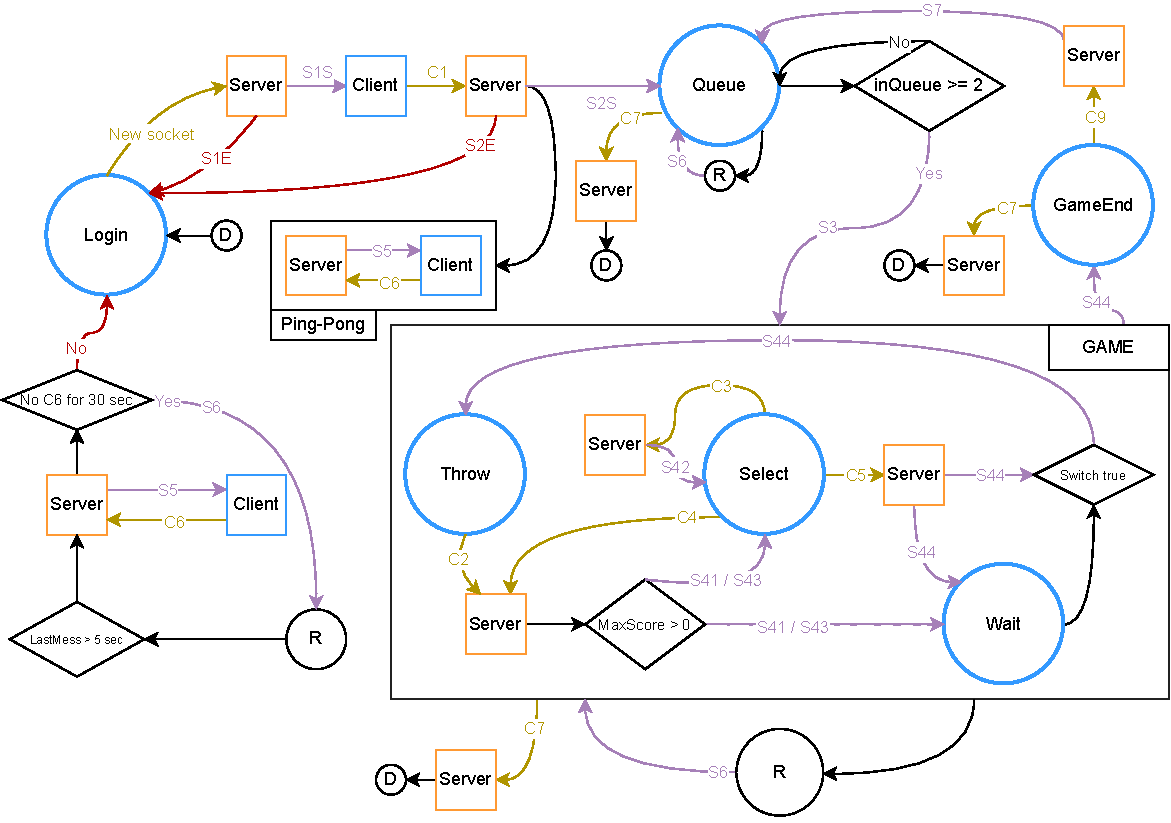
\includegraphics[width=1.3\textheight]{Images/Protocol.drawio.pdf}
        \caption{Diagram protokolu}
        \label{fig:diagram}
    \end{figure}
\end{landscape}

\newpage

\section{Implementace}
\subsection{Server}
Server je implementován v~jazyce C++ s~využitím BDS socketů pro komunikaci s~klientem a~standardní knihovny pro zpracování zpráv.
Celý server je rozdělen do několika modulů:
\begin{itemize}
    \item Main -- Hlavní modul.
    \item Server -- Modul pro komunikaci s~klientem.
    \item Messages -- Modul pro zpracování zpráv a~generací odpovědí.
    \item Data -- Modul pro ukládání dat.
    \item Events -- Modul pro zpracování událostí.
    \item Utils -- Modul pro pomocné funkce.
\end{itemize}

\subsubsection{Main}
Hlavní modul obsahuje inicializaci serveru a~jeho běh.
Načítá IP a~port z~příkazové řádky a~spouští server.
Dodatečně spouští vlákno pro zpracování příkazu nad serverem.
Příkazy:
\begin{itemize}
    \item \textbf{exit} -- Ukončení serveru.
    \item \textbf{help} -- Vypsání nápovědy.
    \item \textbf{players} -- Vypsání seznamu připojených klientů.
    \item \textbf{games} -- Vypsání seznamu her.
    \item \textbf{all} -- Vypsání všech dat.
\end{itemize}

\subsubsection{Server}
Modul pro komunikaci s~klientem.
Zde se server zinicializuje, naslouchá na zadaném portu a~přijímá nové klienty.
Pro zpracování byly využit Select a~BDS socket.
Každý klient tedy má svoje fd neboli file descriptor.
Všichni klienti jsou zpracováni v~jednom vlákně.
Po kontrole všech fd se zpracují speciální události 
(nová hra, smazání hry, odpojení klienta, update, znovu připojení klientů do hry).

Dále zde běží vlákno pro zjištění živosti klienta.
Klient každé 3~sekundy pošle pong a~server odpoví ping.
Pokud klient nepošle ping do 5~sekund, server se zeptá, jestli klient žije.
Pokud klient neodpoví do 30~sekund je odpojen.

Čtení zprávy má dvě fáze:
Načtení hlavičky a~načtení zbytku zprávy.
Po načtení hlavičky se zkontroluje, zda je zpráva validní.
Pokud ano načte se zbytek zprávy a~zpracuje se.
Pokud ne, je klient odpojen.

Zpracování zpráv je delegováno do modulu Messages.

\subsubsection{Messages}
Modul pro zpracování zpráv a~generování odpovědí.
Z~přečtené zprávy se zjistí tag a~data.
Tag se vyhledá v~unordered mapě a~zavolá se příslušná funkce.
Pokud tag není nalezen, je zaslána zpráva, která klienta odpojí.
Zprávy jsou do jednotlivých modulů, pokud se jedná o~
Login, Logout, Reconnect, RejoinQ a~GameM (Všechny zprávy týkající se hry).

\subsubsection{Data}
Modul pro ukládání dat.
Zde jsou uloženy všechny informace o~hrách, hráčích a~herních objektech.

Objekt \textbf{hráč} obsahuje:
\begin{itemize}
    \item Jméno hráče.
    \item File descriptor.
    \item Stav hráče určen číslem:
    \begin{itemize}
        \item[>] -2 -- Hráč bez jména.
        \item[>] -1 -- Odpojený hráč s~možností se vrátit.
        \item[>] 0 -- Hráč v~Queue.
        \item[>] 1 -- Hráč ve hře.
    \end{itemize}
    \item Poslední aktivita (pro kontrolu živosti).
\end{itemize}

\newpage
Objekt \textbf{hra} obsahuje:
\begin{itemize}
    \item Vector hráčů.
    \item Vector jmen hráčů.
    \item onMove -- Jméno hráče na tahu.
    \item Vector Vektorů kostek.
    \item Vector Vektorů skóre.
    \item bool end -- Konec hry.
    \item bool stop -- Zastavení hry.
\end{itemize}
Tento objekt má dále metody pro funkce hry.

Objekt \textbf{kostka} obsahuje:
\begin{itemize}
    \item Id kostky.
    \item Hodnotu kostky.
    \item Vybraná kostka.
    \item Držená kostka.
\end{itemize}
Dále má metody pro zpracování kostek (Roll, Select, Hold).

Objekt \textbf{DataVectors} obsahuje 2~vektory pro ukládání všech her a~hráčů.

\subsubsection{Events}
Modul pro zpracování událostí.
Jedná se o~události:
\begin{itemize}
    \item Nová hra -- Vytvoření nové hry.
    \item Reconnect -- Připojení odpojeného hráče do hry.
    \item Oznámení, zda byl klient odpojen nebo připojen.
\end{itemize}

\subsubsection{Utils}
Modul pro pomocné funkce.
Nachází se zde funkce pro počítání skóre a~zpracování příkazů nad serverem.
Dále je zde soubor \texttt{Consts.h} s~konstantami pro server.

\newpage
\subsection{Klient}
Klient je implementován v~jazyce Java s~využitím knihovny Swing pro grafické rozhraní.
Celý klient je rozdělen do několika modulů:
\begin{itemize}
    \item Main -- Hlavní modul.
    \item GameObjects -- Modul pro herní objekty.
    \item GUI -- Modul pro grafické rozhraní a~zpracování příchozích zpráv.
    \item Server -- Modul pro komunikaci se serverem.
    \item Utils -- Modul pro pomocné funkce.
\end{itemize}

\subsubsection{Main}
Hlavní modul obsahuje inicializaci klienta a~jeho běh.

\subsubsection{GameObjects}
Modul pro herní objekty.
Třídy Board Dice a~PlayerStats obsahuje potřebné funkce pro vykreslení herního pole.
Zatím co Board je jen vykreslení Dice a~PlayerStats obsahují i~pár proměnných pro zpracování dat.

\subsubsection{GUI}
Modul pro grafické rozhraní a~zpracování příchozích zpráv.
Nachází se zde 4~panely:
\begin{itemize}
    \item LoginPanel -- Panel pro přihlášení.
    \item QueuePanel -- Panel pro čekání ve frontě.
    \item GamePanel -- Panel pro hru.
    \item HelpPanel -- Panel pro nápovědu.
\end{itemize}

Všechny panely, kromě GamePanelu používají GridBagLayout pro rozložení prvků.
GamePanel používá funkčnost Graphics2D pro vykreslení hry.
Ovládání je pomocí klávesnice s~využitím InputMap a~ActionMap.

\newpage
\subsubsection{Server}
Modul pro komunikaci se serverem.
Obsahuje třídu Connection, která je navržena jako Singleton.
Po vyplnění údajů v~LoginPanelu se otevře socket a~začne komunikace se serverem.
Pokaždé, co je třeba poslat zprávu se zavolá metoda makeContact, která sestaví zprávu a~odešle ji.
Příchozí zprávy jsou čteny v~samostatném vlákně.
Pokud je zpráva validní zpráva projde dál do GUI pro zpracování.
Dále zde běží pingovací vlákno pro životnost klienta.
Po 5~sekundách co nepřišla zpráva se registruje odpojení a~po 30~sekundách se klient vrátí na Login.
Dále je zde třída Messages, která obsahuje všechny zprávy, které mohou být poslány ze serveru nebo klienta.

\subsubsection{Utils}
Modul pro pomocné funkce.
Nachází se zde soubor \texttt{Consts.java} s~konstantami pro klienta.
Dále \texttt{Colours.java} s~barvami pro GUI a~objekty.
Třída \texttt{Materials.java} obsahuje načítání textur pro objekty

\newpage

\section{Uživatelská příručka}
\subsection{Server}
Server může být spuštěn pouze na Linuxu.
Pro přeložení a~spuštění serveru je třeba mít nainstalovaný g++ a~make.
\begin{itemize}[itemsep=-4pt]
    \item \textbf{Přeložení:} \texttt{make}
    \item \textbf{Spuštění:} \texttt{./Dice\_Server}
    \item Po spuštění zadat IP a~port do příkazové řádky.
\end{itemize}

\subsection{Klient}
Klient může být spuštěn na Windows, Linuxu a~MacOS.
Pro přeložení je třeba mít nainstalovaný JDK 17~a~Apache Maven.
\begin{itemize}[itemsep=-4pt]
    \item \textbf{Přeložení:} \texttt{mvn package}
    \item \textbf{Spuštění:} \texttt{java -jar target/Dice\_Client-1.0-SNAPSHOT.jar}
\end{itemize}

Průchod hrou:
\begin{itemize}
    \item Po spuštění zadat Jméno, IP a~port do GUI (výchozí je 127.0.0.1~a~10000).
    \item Po připojení se zobrazí Queue, kde čekáte na hru.
    \item Po připojení druhého hráče se zobrazí Game.
    \item Ovládání je pomocí klávesnice.
    \begin{itemize}[itemsep=-4pt]
        \item \textbf{Space} -- Hod kostkami.
        \item \textbf{A} -- Pohyb mezi kostkami doprava.
        \item \textbf{D} -- Pohyb mezi kostkami doleva.
        \item \textbf{E} -- Vybrání kostky.
        \item \textbf{F} -- Další hod.
        \item \textbf{Q} -- Ukončení kola.
        \item \textbf{T} -- Nápověda. 
    \end{itemize}
    \item Po skončení hry se zobrazí výsledek, kdo vyhrál a~můžete se vrátit do Queue nebo se odpojit.
    \item Po odpojení se zobrazí Login.
    \item Pokud se oponent odpojí můžete se vrátit do Queue a~čekat na oponentův návrat.
\end{itemize}

\newpage
\section{Závěr}
Cíle práce byly splněny.
Byla vytvořena síťová hra Kostky (Farkle) pro dva hráče.
Pokud jste teď dohráli hru Kingdome Come: Deliverance, můžete si zahrát tuto hru s~přáteli.
Ovšem není to přesná kopie, ale spíše inspirace.
Bylo by možné přidal možnosti pro více typů kostek (např. lichá a~sudá kostka).


\end{document}
